\subsection{Variance reduction}
\subsubsection{Cell-based biasing}
\label{sec:vr:cell}

Cell-based weight window can be generated with the following arguments:

\lstinputlisting[language=bash,numbers=none,backgroundcolor=\color{yellow!20},frame=tb]{UserGuide/cell-biasing.sh}

\begin{description}
\item[-defaultConfig Single ODIN -angle objAxis odinAxis 0] These optional arguments build the ODIN beam line
  and rotate geometry around the $z$ axis in such a way that ODIN is collinear to the $x$ axis.
  This rotation simplifies the weight window source plane setup for the current example and used here for
  illustration purpose~(see \figref{fig:vr:cell}).
\item[-w] should precede all weight-related arguments.
\item[--weightEnergyType] defines energy grid\footnote{With the {\tt wwg} card you can either use this expression or {\tt --wwgE}.}.
  The following variants of syntax are possible:
  \begin{enumerate}
    \item If use the word {\em energy} then the format is energy followed by default weight for that bin
      (in our example: for energies below \SI{0.1}{\mega\electronvolt} the default weight is \num{0.95};
          for energies between \num{0.1} and \SI{1}{\mega\electronvolt} the default weight is \num{0.85} etc).
    \item If you drop the word {\em energy} then you just set the energy grid without specifying default weights.
    \item Alternatively you can use pre-defined keywords:
      {\tt basic}, {\tt high}, {\tt mid} and {\tt flat}\footnote{Energy-weight binnings for these keywords are defined in \tt{System/weights/WeightControl.cxx}}.
    \end{enumerate}
\item[--weightSource] This argument defines a point in space. We can define as many as we want (by adding several {\tt weightSource} arguments),
  but only those used with {\tt weightObject} will be used.
  This particular point is shown by a circle in the left side of \figref{fig:vr:cell:labels}.
\item[--weightPlane] This argument defines a plane. Similarly to {\tt weightSource}, we can define as many planes as we want,
  but only those used with {\tt weightObject} will be used.
  This particular plane is shown by a dashed vertical line in the right side of \figref{fig:vr:cell:labels}.
\item[--weightObject] Define objects we would like to make cell-based variance reduction to.
  \begin{description}
  \item[G2BLineTop20] Object name.  It's also possible to specify range of objects within an object or cell name via {\tt CellMap}.
    \item[SS0] Refer to the first simple source term (the point defined via {\bf weightSource} above)  % 00:10
    \item[energyCut=0.0] Energy cut. Defines min energy for variance reduction (i.e. no variance reduction below this energy will be made~--- default weight will be used \alert{The weight defined in weightEnergyType?}).
    \item[scaleFactor=1.0] Linear scale factor. You are going to work out an exponent which is the scattering term into something. It's $\exp(-\sigma \rho / r^2)$.
      It's transport to go from {\em a} cell to another cell. \alert{Scale factor is taken out in the mesh based variance reduction.}
    \item[density=0.9] Density scale factor. Normally we set it a bit less than one to make it easier to do transport through thick layers.
    \item[r2Len=1.0] Length scale factor \alert{Do not understand}
    \item[r2Pow=2.0] Scale for the length exponent in $r^{\text{r2Pow}}$.
  \end{description}

 % {\tt TP1}: tally plane 1;
 %  \mbox{\tt 1.0 1.0 0.15 1e-20}: energy above \SI{1}{\mega\electronvolt} (below it we are not interested~--- use default values);
 %  {\tt 1.0}: scale factor; 
 %  {\tt 0.15}: density factor; {\tt 1e-20}: minimum weight % 41:12
\item[--voidUnMask] By default the importance of the void cell surrounding geometry is 0. This argument sets it to 1.
  It can be useful if we believe that particles travelling through that cell can contribute into the tally.
  It's always recommended to put this flag unless you really understand what you are doing.
\end{description}

\paragraph{Notes}
\begin{itemize}
\item In order to set up biasing, you need at least one source and one tally. If several tallies are used, then the previous tally is called {\em joint} and servers as a source for the current one.
\item Source can be defined either as a point (via {\bf --weightSource}) or a plane (via {\bf --weightPlane}). In the example above we defined point source.
  However the defined sources and planes do nothing until you use them in {\bf --weightObject} or somewhere else.
\item General rule to get the things into work: try different setups and compare results. Then you renormalise it back out again. It's just basically numerical level game.
  Very often SA scales by this and then rescales by that.
\end{itemize}

% \begin{equation}
%   \label{eq:vr:cellweight}
%   W = \exp{(-w \cdot \sigma_{\text{scale}} \cdot \text{scaleFactor} \cdot \text{factor})}
% \end{equation}

% % CellWeight.cxx
% $$
% factor = minW < \num{1e-16} ? log(\num{1e-16})/log(minW) : 1.0
% $$


\begin{landscape}
\begin{figure}
  \centering
  \subfloat[Horizontal view: geometry \label{fig:vr:cell:labels} ]{
  \begin{tikzpicture}
    \node[anchor=south west,inner sep=0] (image) at (0,0) {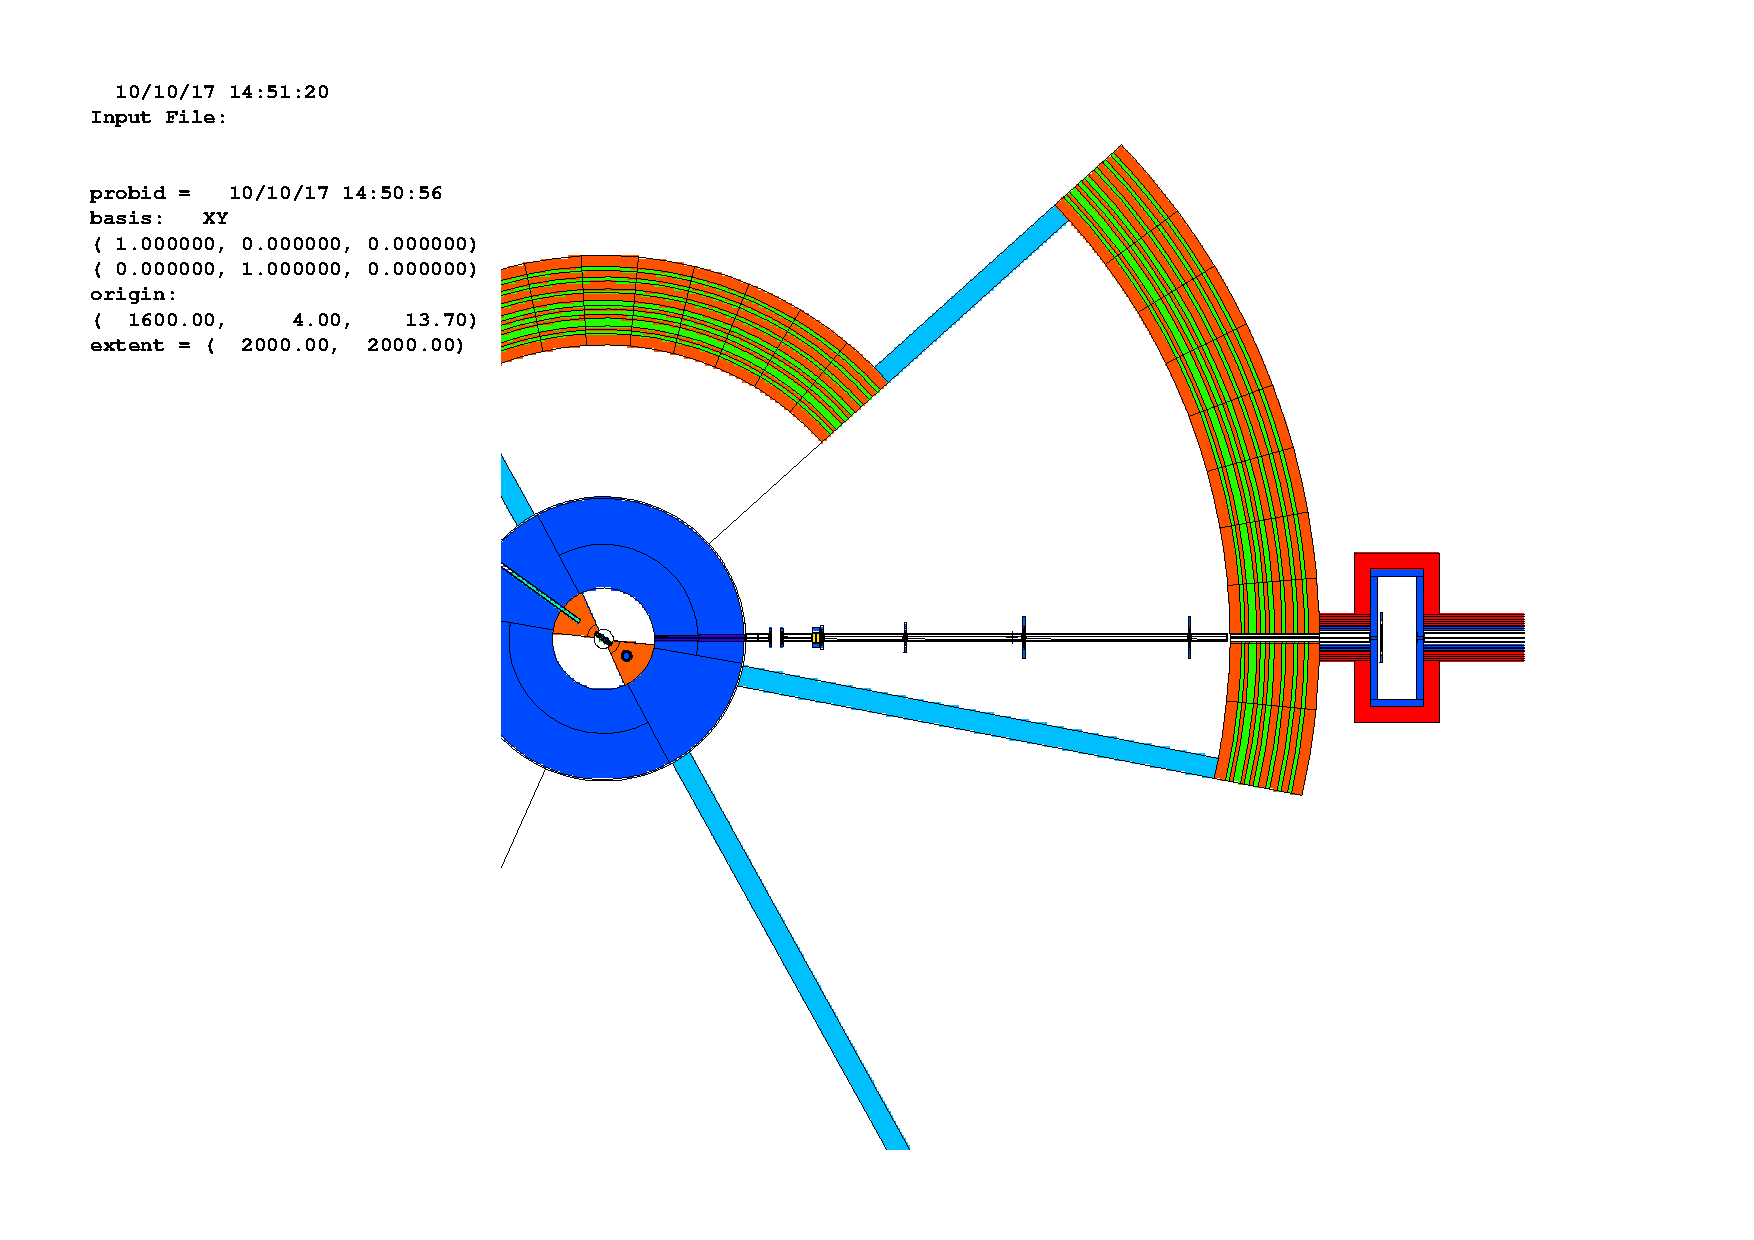
\includegraphics[width=0.5\linewidth,page=1,clip=true, trim=10cm 8cm 4cm 7cm]{UserGuide/cell-biasing.pdf}};
    \begin{scope}[x={(image.south east)},y={(image.north west)}]
      % \draw[help lines, xstep=.1, ystep=.1] (0,0) grid (1,1);
      % \foreach \x in {0,1,...,9} {\node [anchor=north] at (\x/10, 0) {0.\x}; }
      % \foreach \y in {0,1,...,9} {\node [anchor=east]  at (0, \y/10) {0.\y}; }

      \draw[red,thick] (0.07, 0.367) circle (0.5mm);
      \draw[arrow] (0.11,0.46) -- (0.077,0.38);
      \node[legend, anchor=west] at (0.1,0.5) {weightSource};

      \draw[red,dashed] (0.79,0) -- (0.79,1);
      \draw[arrow] (0.85,0.8) -- (0.79,0.8);
      \node[legend, anchor=west] at (0.85,0.8) {weightPlane};

      \draw[arrow]     (0.14,0.2) -- (0.14,0.36);
      \node[legend] at (0.14,0.2) {G2BLineTop20};

      \draw[arrow]                 (0.65,0.25) -- (0.69,0.25);
      \node[legend,anchor=east] at (0.65,0.25) {CBunkerWallMainWall1};

      \draw[arrow]                 (0.65,0.45) -- (0.69,0.45);
      \node[legend,anchor=east] at (0.65,0.45) {CBunkerWallMainWall2};
    \end{scope}
  \end{tikzpicture}
  }
  \subfloat[Horizontal view: wwn]{
    \includegraphics[width=0.5\linewidth,page=2,clip=true, trim=10cm 8cm 4cm 7cm]{UserGuide/cell-biasing.pdf}
  } \\
  \subfloat[Vertical view: geometry]{
    \includegraphics[width=0.5\linewidth,page=3,clip=true, trim=10cm 8cm 4cm 7cm]{UserGuide/cell-biasing.pdf}
  }
  \subfloat[Vertical view: wwn]{
    \includegraphics[width=0.5\linewidth,page=4,clip=true, trim=10cm 8cm 4cm 7cm]{UserGuide/cell-biasing.pdf}
  }
  \caption{Cell-based weight window}
  \label{fig:vr:cell}
\end{figure}
\end{landscape}